\section{Cosmic shear statistics}
\label{sec:theory}

Cosmic shear data can be analysed using various summary statistics, each with its own advantages and disadvantages.
%Cosmic shear data can be analysed by a number of summary statistics, which all have their pros and cons.
We first review the modelling and measurement methods of shear two-point functions, then present other complementary cosmic shear statistics in the second part of this section.

%-------------------------
\subsection{$\gamma$-2PCF}
\label{subsec:wl-th}

\begin{figure}
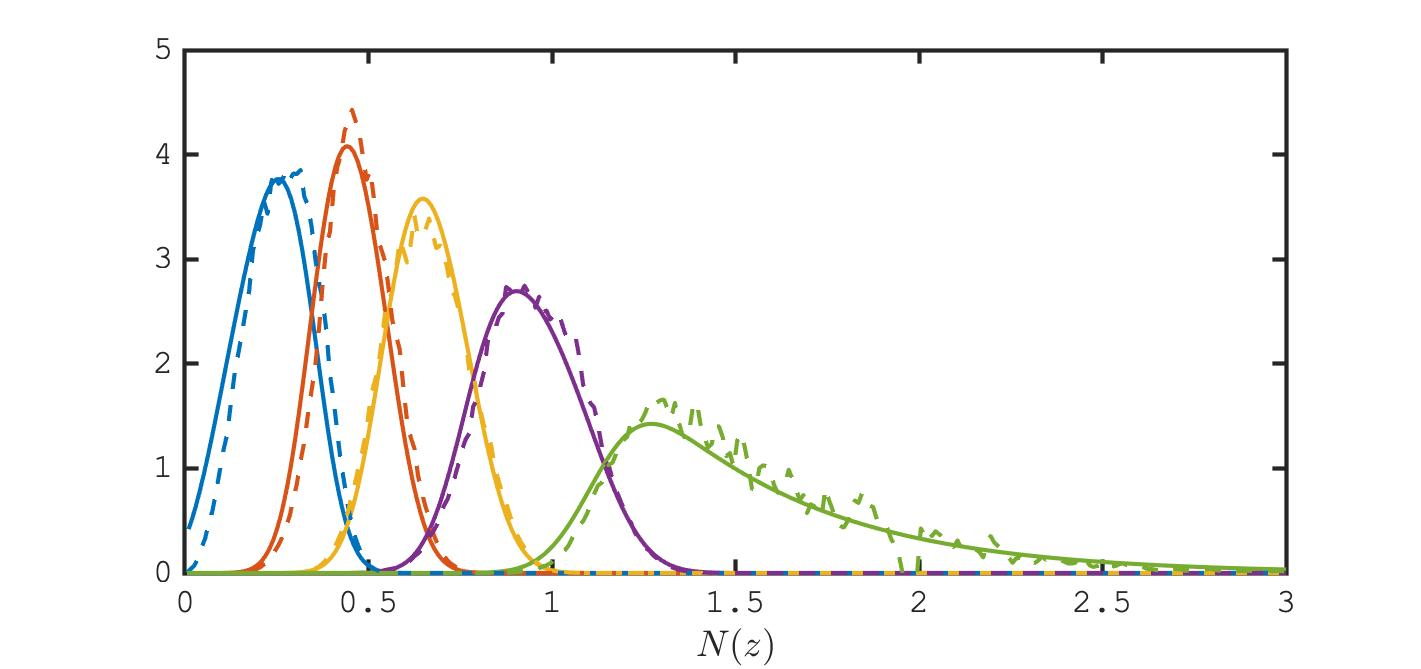
\includegraphics[width=\columnwidth]{graphs/Nz}
\caption{Tomographic redshift distributions in our simulations, either taken from the Year-1 specifications for LSST (solid) or from a matched selection applied to an HOD galaxy catalogue (dashed, see Sec. \ref{subsec:HOD}).}
\label{fig:Nz}
\end{figure}

Shear two-point correlation functions (\gtwopcf hereafter) can be predicted with percent-level precision and are therefore an ideal quantity to validate weak lensing simulations.
In the Limber approximation\footnote{See \citet{Kilbinger17} for a comparison between the Limber approximation and the exact calculations.}, the lensing angular power spectrum $C^{ij}_{\ell}$ (in spherical harmonics space) in tomographic bins $i$ and $j$ is obtained from an integral over the three-dimensional matter power spectrum $P_{\delta}(k, z)$ (in Fourier space, and redshift $z$ dependant):
  \begin{eqnarray}
C_{\ell}^{ij} = \int_0^{\chi_{\rm H}}  \frac{q^i(\chi) \,q^j(\chi)}{\chi^2} \, P_{\delta}\, \bigg(\frac{\ell+1/2}{\chi},z(\chi)\bigg) \ {\rm d}\chi,
\label{eq:C_ell}
\end{eqnarray}
where $\ell$ is a multipole, $\chi_{\rm H}$ is the co-moving distance to the horizon, $c$ is the speed of light, $H_0$ the Hubble parameter, and the lensing kernels $q^{i}$ and $q^j$ are given by:
\begin{eqnarray}
q^{i(j)}(\chi) = \frac{3}{2}\Omega_{\rm m} \, \bigg(\frac{H_0}{c} \bigg)^2 \frac{\chi}{a(\chi)} \int_{\chi}^{\chi_{\rm H}} n^i(\chi')\frac{{\rm d}z}{{\rm d} \chi'}\frac{\chi' - \chi}{\chi'}{\rm d}\chi' \, .
\label{eq:q_lensing}
\end{eqnarray}
In the previous expression, $n^i(z)$ refers to the redshift distribution  in tomographic bins `$i (j)$', while $a(\chi)$ is the scale factor at co-moving distance $\chi$ from the observer.
For more details, consult \citealt{Lamman_IA_guide}.
The matter power spectrum is computed from  {\sc Halofit} \citep{Takahashi2012} in this work, however other public tools provide accurate predictions, including \eg {\sc HMcode} \citep{HMCode2020}, the {\sc EuclidEmulator} \citep{EuclidEmulator}, the {\sc Bacco} emulator \citep{BACCOEmulator}, or the {\sc MiraTitan} emulator \citep{miraTitan}. 
Predictions for the \gtwopcf are finally computed from Eq. (\ref{eq:C_ell}) as:
\begin{eqnarray}
\xi_{\pm}^{ij}(\theta) = \frac{1}{2\pi} \int_0^{\infty} C_{\ell}^{ij} \, J_{0/4}(\ell \theta) \, \ell \, {\rm d}\ell,
\label{eq:xipm_th}
\end{eqnarray}
where $J_{0/4}(x)$ are Bessel functions of the first kind. 
In this paper, these calculations are carried out by the {\sc CosmoSIS} cosmological inference package \citep{cosmoSIS}.
The redshift distribution $n (z)$ is the source galaxy sample redshift distribution of LSST Year1 \citep{LSST-SRD}:
\begin{eqnarray}
n (z) =  z^2 \: {\rm exp} \left[-\left(\frac{z}{z_0}\right)^\alpha \right]\, ,
\label{eq:nz}
\end{eqnarray}
with pivot redshift $z_0=0.13$ and a power-law index $\alpha = 0.78$.
The distribution is normalised to provide a number density of $n_{\rm eff} = 3.0 $  galaxies per arcmin$^{2}$.
This is a bit lower than the expected number density for the first data release ($n_{\rm eff}\sim10$ galaxies arcmin$^{-2}$), but is large enough to validate our methods, and makes the calculation more tractable.
This global $n(z)$ is further split into five equi-populated tomographic bins, and smoothed with a Gaussian filter of width $\sigma = 0.05 \: (1 + z)$ to mimic the photometric selection process, shown by the solid lines in Fig. \ref{fig:Nz}. 

The weak lensing signal is measured from the ellipticities $\epsilon_{1/2}$ of simulated or observed galaxies, which, in absence of systematics and secondary signals, are unbiased estimators  of the cosmic shear components $\gamma_{1/2}$.
In particular, the \gtwopcf are estimated as:
\begin{eqnarray}
\widehat{\xi_{\pm}^{ij}}(\theta) = \frac{\sum_{a,b} w_a w_b \left[\epsilon_{a, \rm +}^i\epsilon_{b, \rm +}^j     \pm \epsilon_{a, \times}^i\epsilon_{b, \times}^j    \right]\Delta_{ab}(\theta)}{\sum_{a,b} w_a w_b} \, ,
\label{eq:2PCF_estimator}
\end{eqnarray}
where the sum is over all pairs of galaxies $a, b$ separated by an angular distance $\theta$ on the sky, respectively belonging to the tomographic bins $i$ and $j$.
$w_{a (b)}$ represent the projected correlation functions, while the tangential/cross components of ellipticities are denoted as $\epsilon_{+/\times}$, respectively. 
$\Delta_{ab}(\theta)$ is the binning operator, equal to unity if the angular separation between the two galaxies falls within the $\theta$-bin, and zero otherwise, while the shape weights $w_{a,b}$ are set to unity.
In this work, we construct lensing catalogues from numerical simulations (described in Sec. \ref{sec:sims}), from which we measure $ \widehat{\xi_{\pm}^{ij}}(\theta)$ with {\sc Treecorr} \citep{TreeCorr}.
We set therein the {\sc bin\_slop} parameter to 0.05, then compute the correlations in 20 logarithmically-spaced angular bins with outer edges ranging from $0.5$ to $475.5$ arcmin. 
 
 
 %-------------------------
\subsection{Non-Gaussian lensing statistics}
\label{subsec:beyond-2pt}

Non-Gaussian statistics have the potential to extract cosmological information stored in the complex phases of the density field, outperforming in that sense the \gtwopcf that can only access information encoded in the complex amplitudes.
No optimal estimator has been identified to-date as being able to capture `all' information, but numerous studies all show a clear gain in constraining power, especially when used in combination with two-point functions \citep{HD21, DESY3_Zuercher, HSC_PeaksSims}.
While some of these act on galaxy catalogues directly, many non-Gaussian statistics are measured on convergence or aperture mass maps, requiring the post-process the galaxy catalogues with a mass-reconstruction algorithm.
To accommodate a variety of cases, we therefore provide both galaxy catalogues and convergence maps, the latter being  produced from the galaxies' observed ellipticities with the standard Kaiser \& Squires inversion technique \citep{KaiserSquires}.
These are spherical {\sc Healpix}\footnote{{\sc Healpix}: http://healpix.sf.net}  maps \citep{healpix} with $N_{\rm side}=4096$ generated over an octant, and includes a baseline $2.0$ arcmin smoothing beam to suppress numerical noise.

It's worth noting that this smoothing scale is relatively small, posing challenges for theoretical modeling of some probes within this regime.
Consequently, modeling often requires direct inference from simulations \citep[see][]{HD21, DESY3_Zuercher, HSCY1_Peaks_sims}.
%Note that this smoothing scale is quite small; some probes are difficult to model theoretically in that regime, in which case the modelling needs to be inferred from simulations directly \citep[as in][]{HD21, DESY3_Zuercher, HSCY1_Peaks_sims}.
In the interest of brevity, this paper does not cover statistics derived from aperture mass maps, though our methods are equally applicable to those estimators.
%We do not discuss statistics based on aperture mass maps in this paper for the sake of conciseness, but all our methods can be applied to those estimators as well.
While tomographic \gtwopcf data include auto-correlation and cross-redshift correlations, certain non-Gaussian statistics extract further information from analyzing triplets, quadruplets, or quintuplets of redshift bins \citep{Martinet21a}.
This work focuses only on auto-tomographic bins, yet our methods and results can be straightforwardly extended to accommodate such analyses.

%Whereas tomographic \gtwopcf data consists of auto-correlation and cross-redshift correlations, some non-Gaussian statistics can learn additional information from analysing catalogues or maps constructed from triplets, quadruplets or quintuplet of redshift bins \citep{Martinet21a}. 
%We do not fully exploit this possibility here and consider auto-tomographic bin only, nevertheless all of our methods and findings can be easily generalised to include this. 
 
 
\subsection{Catalogue-based statistics}

A number of higher-order statistics work at the level of shear catalogue,  and here we consider the following:
\begin{enumerate}
\item {\it Three-point correlation functions (or $M_{\rm ap}^3(\theta)$)}:  \JHD{ Lucas/Laila, can you summarise the measurements and modelling, and provide references?}
\item {\it Squeezed bispectrum}: \JHD{ Anik, can you summarise the measurements and modelling, and provide references?}
\end{enumerate}

\subsection{Convergence-based statistics}

We further consider the following convergence map-based statistics:
\begin{enumerate}
    \item \textit{Convergence three-point correlation function}: \JHD{Alejandro, can you summarise the measurements and modelling, and provide references?}
    \item \textit{Peaks and Minima}: local maxima and minima in the {\sc Healpix} convergence maps are counted in bins of signal-to-noise ratios, $\nu$, computed from the global level of shape noise in the survey. 
    These are amongst the most widely used non-Gaussian lensing statistics, as it is simple to measure yet highly sensitive to non-Gaussian structures.
    Although some theoretical models have been developed to describe the largest peaks \citep[see][]{Shan18, HSCY1_Peaks_th}, we report here the results on a much wider range of statistics, which can only be accurately modelled from numerical simulations.
    \item \textit{Lensing PDF}:  \JHD{Cora/Lina, can you summarise the measurements and modelling, and provide references?}
    \item  \textit{Minkowski functionals}: \JHD{Nisha, can you summarise the measurements and modelling, and provide references?}
\end{enumerate}

These statistics explore various physical scales and nonlinear phenomena, leading to differences in their sensitivity to cosmology and systematic errors.
For instance, a statistical method effective in recovering cosmological information could be significantly influenced by secondary effects like intrinsic alignments (IA), casting doubts on its robustness.
Thus, incorporating IA simulations at the field level is essential for addressing these concerns.

 %Each of these statistics probe different physical scales and nonlinearities, causing their sensitivities to cosmological and systematics to vary. 
% For example, a probe that is performing well at recovering cosmological information might be heavily affected by secondary signals such as IA and therefore deemed not robust.
%Having infused IA mocks at the field-level is therefore critical to answer such questions.